%!TEX program = xelatex

\documentclass[cn,black,9pt,normal]{elegantnote}
\usepackage{float}
\usepackage{hyperref}


%\newcommand{\upcite}[1]{\textsuperscript{\textsuperscript{\cite{#1}}}}

\title{数码摄影作业(02)同一对象的两张照片\\\small{同济大学四平路图书馆}}
\author{姓名:姜文渊\\学号:1951510}
%\institute{School of Life Science, Tongji University}
%\version{1.00}
\date{2021年3月19日}

\begin{document}

\maketitle


\section*{使用的器材简介}

下面两张照片是学生所摄的同济大学四平路校区图书馆,
借以展现该图书馆的建筑风格。使用的相机为佳能M200,镜头为\texttt{EF-M15-45mm f/3.5-6.3 IS STM}。

\section{所摄照片}
\begin{figure}[H]
    \centering
    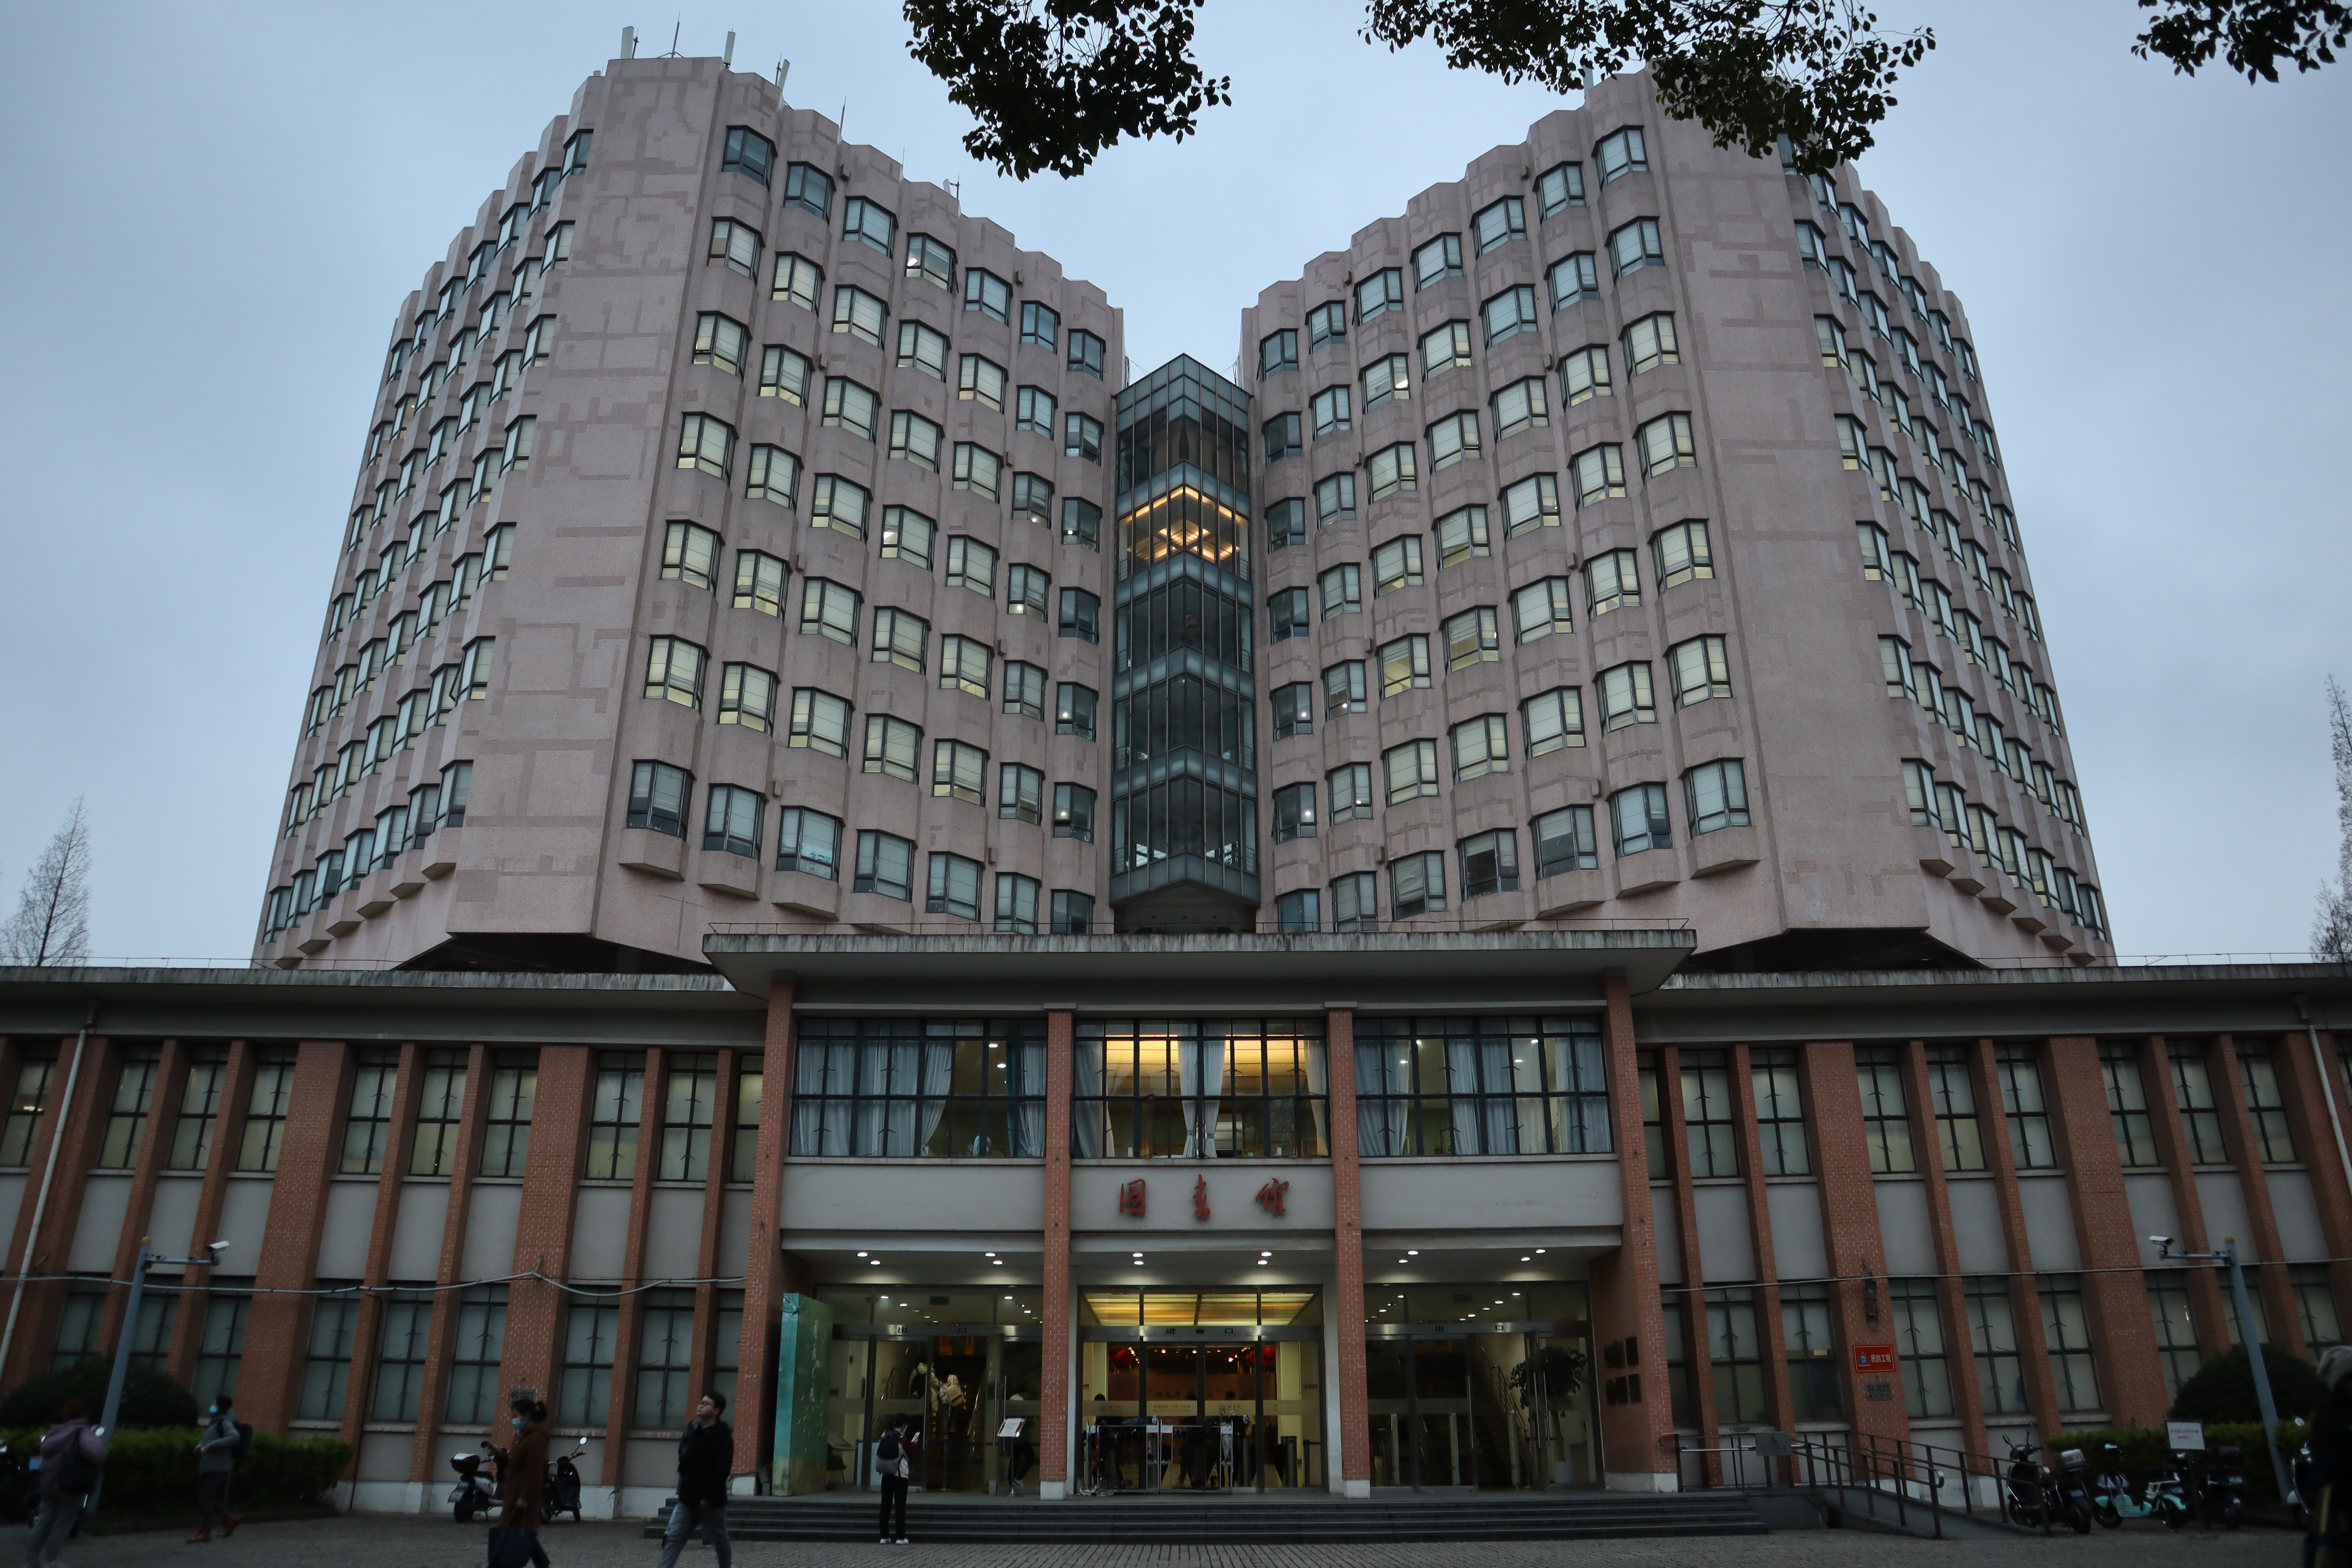
\includegraphics[width=1\textwidth]{IMG_0134.JPG}
    \caption{15mm 1/80 F3.5 ISO 250}
    \label{F-01}
\end{figure}

上面的照片视角较广,可以展现图书馆的全貌,由于拍摄所用为仰视的视角,更显示图书馆的高大。
\section{所摄照片}
\begin{figure}[H]
    \centering
    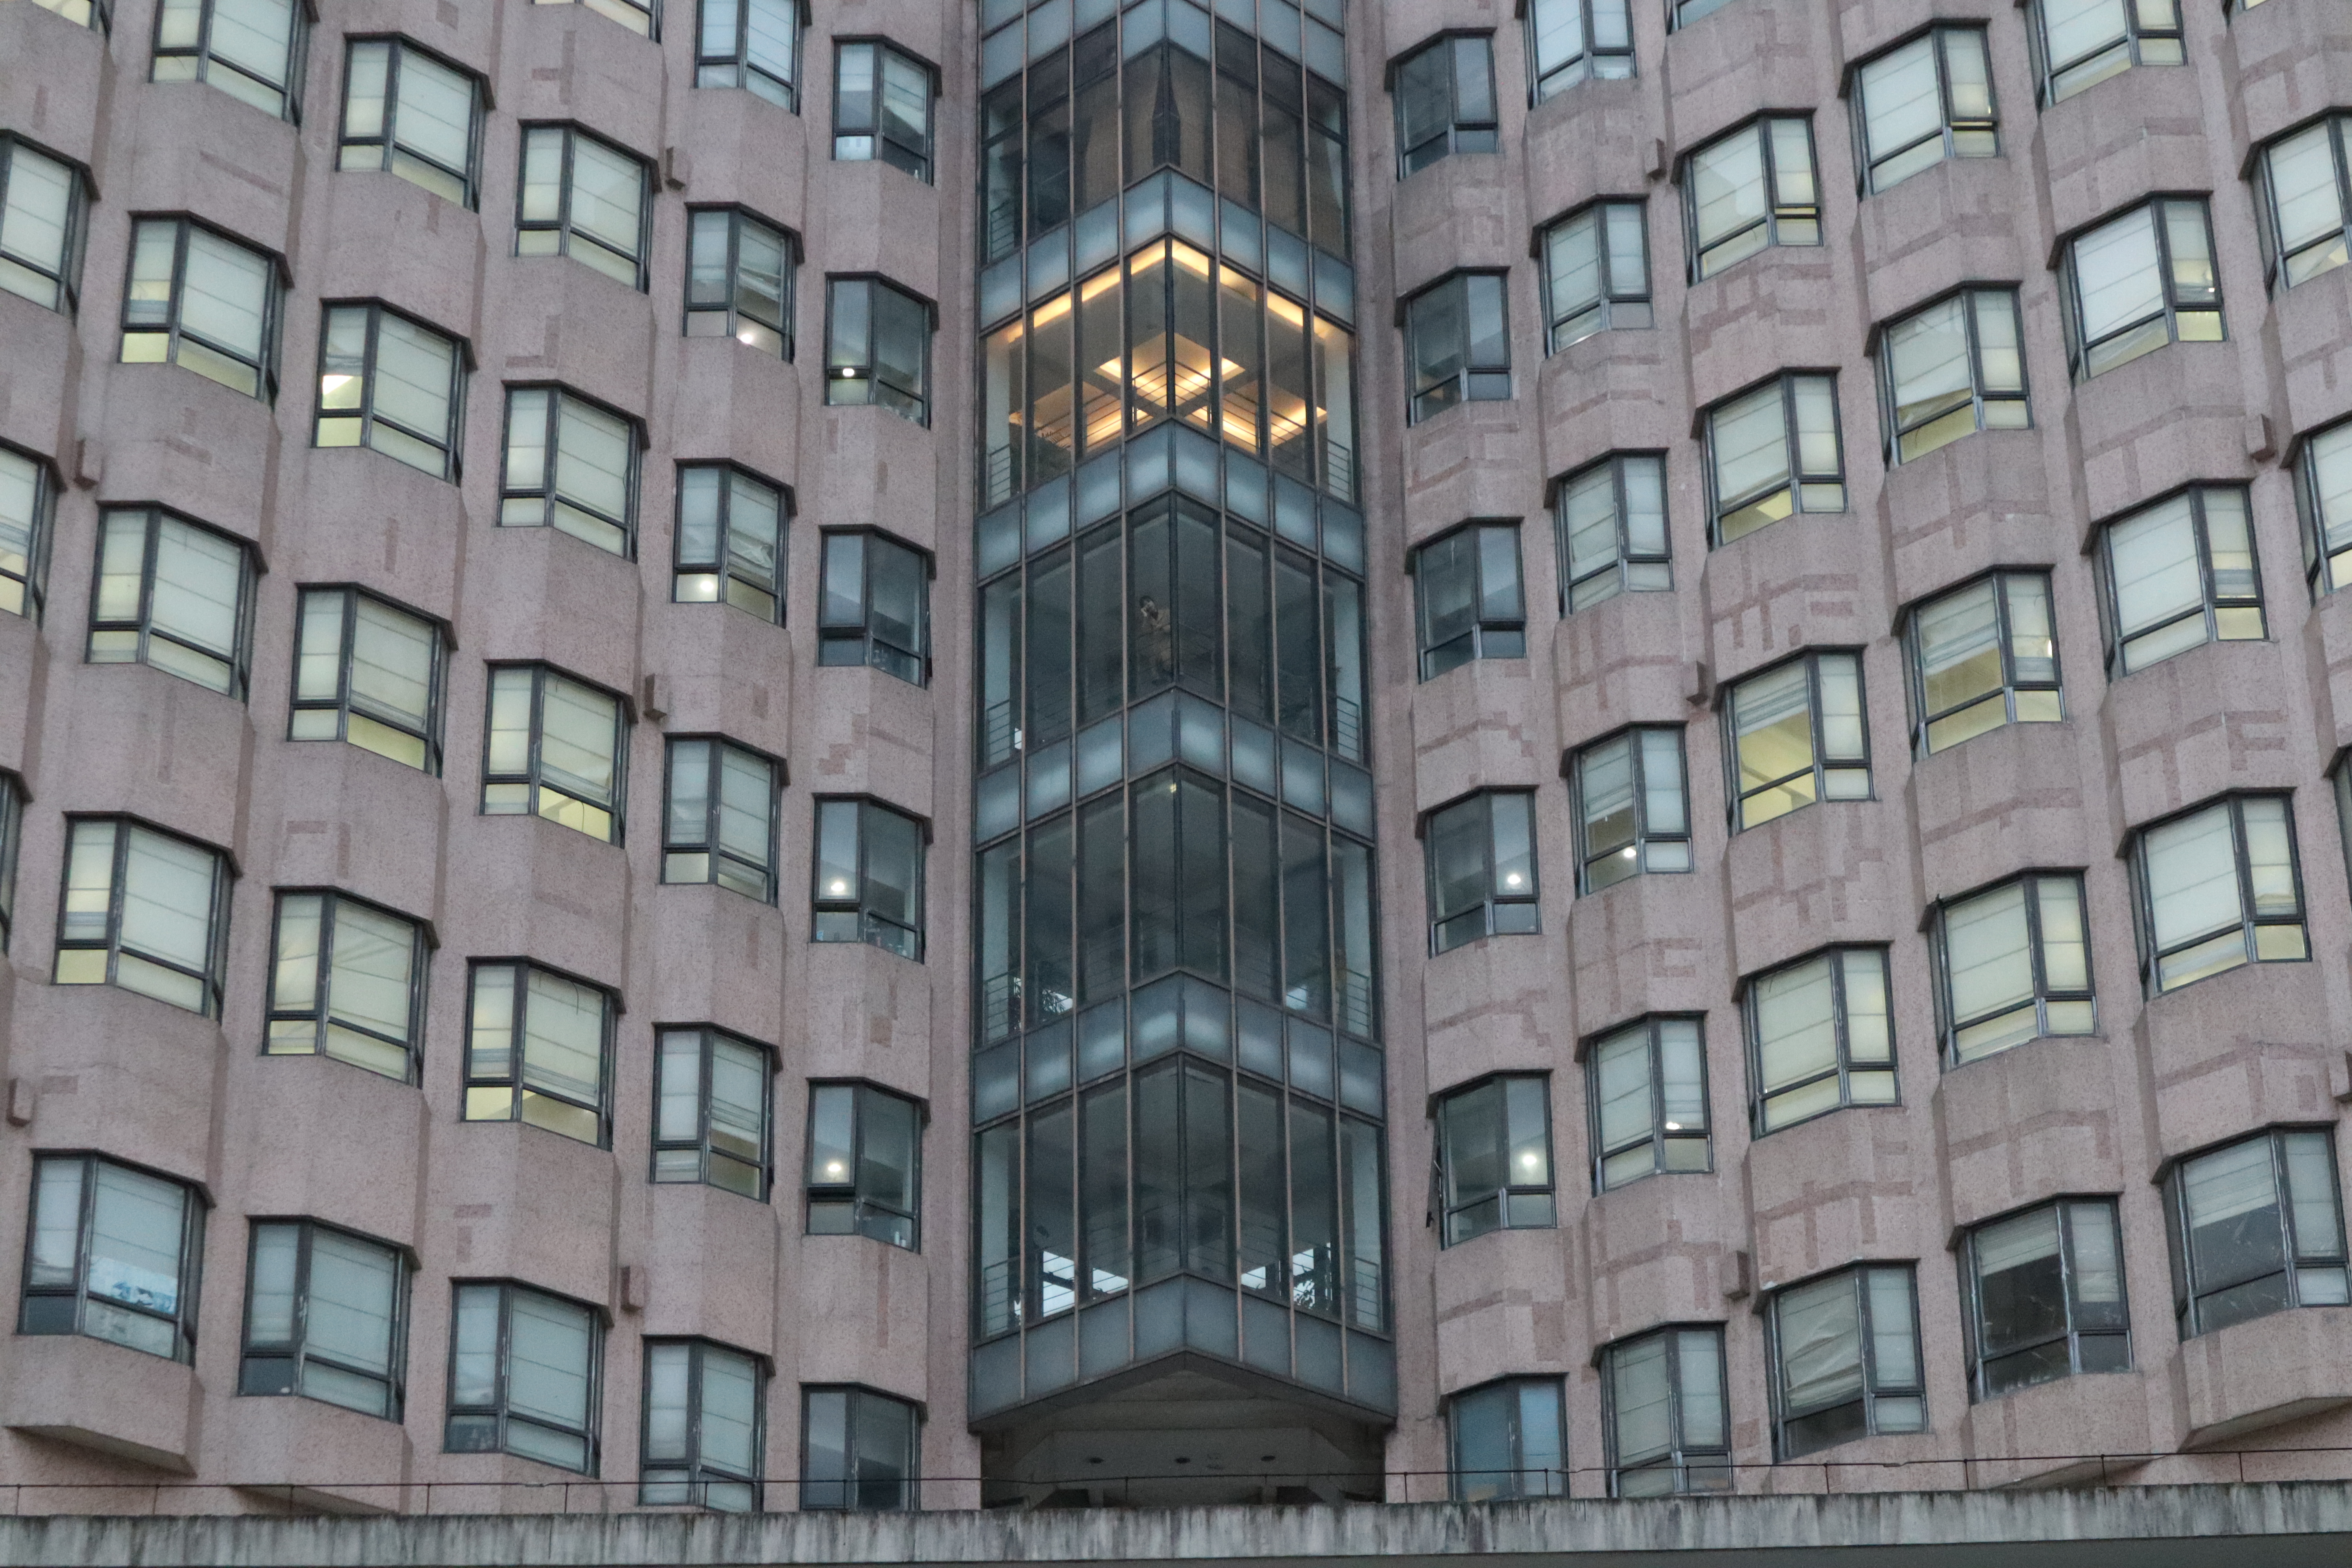
\includegraphics[width=1\textwidth]{IMG_0135.JPG}
    \caption{45mm 1/160 F3.5 ISO 5000}
    \label{F-02}
\end{figure}

而这张照片由于视角较小,展现图书馆外壁的规则的设计,有对称规律的美感。

%\bibstyle{unsrt}
%\bibliography{references}{}
\end{document}
